\documentclass[10pt,onecolumn]{article}


%Aquí vienen todos los paquetes que se van a usar

\usepackage[spanish]{babel}
\usepackage[letterpaper,top=2cm,bottom=2cm,left=3cm,right=3cm,marginparwidth=1.75cm]{geometry}

\usepackage[bottom]{footmisc}
\usepackage{comment}

\usepackage{subcaption} % Añade esto en el preámbulo si no lo tienes
\usepackage{colortbl} %Permite agregar color a las celdas de las tablas.
\usepackage{mathtools} %Contiene herramientas adicionales para componer fórmulas matemáticas en LaTeX.
\usepackage{algorithm2e} %Facilita la sintaxis de los algoritmos.
%\usepackage[T1]{fontenc} %Hace posible escribir en diferentes idiomas.
\usepackage{lmodern} %Carga la fuente Latin modern en el documento.
\usepackage{float} %Hace posible el uso de [H] en las tablas y gráficas.
\usepackage{blindtext} %Ncesario para usar este tipo de comentarios.
\usepackage{multicol} %Posibilidad (no mostrada aquí) de escribir en varias columnas para una misma página.
\usepackage{wrapfig} %Permite que las figuras y tablas se ajusten mejor al texto.
\usepackage{breqn} %Ajusta ecuaciones largas al ancho de la página, teniendo que romper y bajar a una fila más abajo parte de la ecuación para que quepa dentro de los márgenes.
\usepackage{array} %Permite personalizar más ampliamente las columnas de las tablas de LaTeX.
\usepackage{eurosym} %Posibilidad de usar el símbolo € en el texto.
\usepackage{amsmath} %Mejoras para la escritura de ecuaciones matemáticas.
\usepackage{mathrsfs} %Prporciona el alfabeto de letras minúsculas de Ralph Smith.
\usepackage{indentfirst} %Encaja el primer párrafo de un encabezado del documento, si por ejemplo el primer párrafo queremos que esté sangrado.
\usepackage{amsthm} %Facilita la escritura de demostraciones de afirmaciones matemáticas de toda clase.
\usepackage[font=small,labelfont=bf]{caption} %Formatea los títulos de figuras y gráficas.
\usepackage{graphicx} %Facilita la inclusión de imágenes en LaTeX.
\usepackage[titles]{tocloft} %Posibilidad de personalizar el formato del Índice.
\usepackage[hidelinks]{hyperref} %Crea hipervínculos en el PDF generado del documento de texto final, para poder navegar a través y externamente al documento.
\setlength{\parindent}{12pt} %Establece la sangría de la primera línea de cada párrafo a {...pt}.
\usepackage{multirow} %Posibilidad de combinar filas de las tablas de LaTeX.
\usepackage{parskip} %Modifica los espacios entre párrafos para que no haya sangría, sino que se genere un espacio entre medias predeterminado. 
\usepackage{fancyhdr} %Creación de encabezados y pies de página.
\usepackage[utf8]{inputenc} %Permite usar caracteres especiales y letras acentuadas directamente en el código LaTeX.
\usepackage{bm} %Posibilidad de escribir símbolos en negrita en lenguaje matemático. 
\usepackage{url} %Inclusión de direcciones URL en el documento.
\usepackage{siunitx} %Permite la escritura de cantidades físicas y unidades en el documento.
\usepackage{geometry} %Posibilidad de personalizar las dimensiones del documento.
\usepackage{graphicx}
\usepackage{hyperref}
\usepackage{titlesec}


%Aquí se definen cosas de colores y movidas fancys
\usepackage[dvipsnames]{xcolor}
\definecolor{nube}{RGB}{188,108,37}
\definecolor{salmon}{RGB}{248, 131, 121}

%Aquí tenemos un poco el formateo de la página
\pagestyle{fancy}
\fancyhf{}
\cfoot{}
\rhead{\thepage}
 \lhead{Simulación Schrödinger para el oscilador armónico cuántico.}


\begin{document}
\renewcommand{\headrulewidth}{0.5pt}
\newcommand{\HRule}[1]{\rule{\linewidth}{#1}}
\renewcommand{\refname}{Bibliography}
\renewcommand{\tablename}{Table}
\renewcommand{\contentsname}{Index}
\renewcommand{\figurename}{Fig.}
\captionsetup{labelfont={color=nube}}
\addtocontents{toc}{\hspace{-7.5mm} \textbf{Chapters}}
\addtocontents{toc}{\hfill \textbf{Page} \par}
\addtocontents{toc}{\vspace{-2mm} \hspace{-7.5mm} \hrule \par}

\onecolumn
\begin{titlepage}
\centering
    {\HRule{2 pt}} \\
    \vspace{0.5cm}
    {\scshape\Huge Simulación de la ecuación de Schrödinger dependiente del tiempo para el oscilador armónico cuántico.}  \\
    %AQUI SE PONE EL TITULO
    \vspace{1 mm}
    
    {\HRule{2 pt}}

    \vspace{1cm}
    \Large 15/05/2026 \\
    \vspace{1cm}
 
    \normalfont\Large Universidad de Granada, Facultad de Ciencias \\
    \vspace{0.5cm}
    
    
     \normalfont\Large Grado en Físicas \\
    \vspace{0.5cm}
     \normalfont Física Computacional \\
    \vspace{1.5cm}

\centering
    {
\includegraphics[width=0.5\textwidth]{Image/Misc/UGR-MARCA-01-color.jpg}\par}

\vfill
    \vspace{1cm}
    \scshape\Large Jorge del Rio López\\
    
    \vspace{0.5cm}

\vfill

\end{titlepage}

\selectlanguage{Spanish}

\tableofcontents %único comando para manejar TODO el índice.
\newpage

\HRule{0.5pt} %Controla los márgenes horizontales visibles (líneas) y el grosor de la línea (...pt).

\begin{abstract}
Estudio de la evolución temporal de varias funciones de ondas sometidas a un pozo armónico, empleando el método de Crank-Nicolson para la resolución numérica de ec. de Schrödinger dependiente del tiempo. Las funciones de onda estudiadas incluyen las autofunciones del sistema y una función gaussiana, mostrando así las diferencias entre los estados estacionarios y los estados no estacionarios del sistema. 
\end{abstract}

\section{Introducción}
En este proyecto estudiaremos la evolución temporal de diferentes funciones de onda sometidas a un potencial oscilador armónico, veremos el comportamiento de diferentes variables como la probabilidad, el valor medio de la posición, el valor medio del momento, el valor medio de la energía, etc,  para diferentes funciones de onda, mostrando así las diferencias entre los estados estacionarios y los estados no estacionarios del sistema. Para ello emplearemos el método de Crank-Nicolson para la resolución numérica de la ecuación de Schrödinger dependiente del tiempo, lo que nos permitirá obtener una solución aproximada de la función de onda en cada instante de tiempo a partir de su estado inicial.

Además, compararemos el comportamiento cuántico del sistema con el comportamiento clásico del oscilador armónico, mostrando así las diferencias entre ambos comportamientos y cómo la mecánica cuántica se diferencia de la mecánica clásica en este sistema. Así como el limitede la mecánica cuántica con la mecánica clásica, mostrando cómo el comportamiento cuántico se aproxima al comportamiento clásico en ciertas condiciones.





\section{Presentación del problema}
En la teoría de Mecánica Cuántica el comportamiento de un sistema viene descrito por su función de onda $\Psi(x,t)$, la cual debe cumplir la famosa ecuación de Schrödinger:

\begin{equation}
    i\ \hbar [\dfrac{\partial \Psi(x,t)}{\partial t}] = [-\dfrac{\hbar^2}{2\ m}\nabla^2 + V(x)]\Psi(x,t) = H \Psi(x,t)
\end{equation}

Donde $H$ es un operador hermítico, al trabajar en una sola dimensión el gradiente $\nabla^2$ se transforma en una derivada parcial respecto de la variable a estudiar, en este caso trabajaremos con $x$, por lo tanto el operador $\hat{H}$ quedaría de la siguiente forma:

\begin{equation}\label{eq:Operador_H}
\hat{H} = - [-\dfrac{\hbar^2}{2\ m}\dfrac{\partial^2}{\partial x ^2} + V(x) ]   
\end{equation}

Para evitar trabajar con las constantes que aparecen re escalaremos las coordenadas buscando eliminarlas, para ello $t\rightarrow \hbar\ t$ y $x\rightarrow x\ \dfrac{\hbar}{\sqrt{2m}}$, logrando así convertir $m = 0.5$ y $\hbar = 1$, a partir de aquí trabajaremos con estas coordenadas re escaladas.


El potencial que estudiaremos será un potencial muy conocido en la física, el potencial armónico, con ecuación: $V(x)=\dfrac{\omega^{2}}{4}\,{}(x-x_{0})^{2}$

Si resolvemos la ecuación de Schr. mediante el método de separación de variables\footnote{La resolución se encuentra en el apéndice.} llegamos a la expresión de la solución:
\begin{equation}\label{eq:SolucionFormal}
    \Psi(x,t)= e^{-i\ (t-t_0)\  H}\ \psi(x,t_0)
\end{equation}

En la ecuación \ref{eq:SolucionFormal} se muestra la solución formal de la ecuación de Schrödinger dependiente del tiempo, donde $\psi(x,t_0)$ es la función de onda en el tiempo inicial $t_0$ y $e^{-i\ (t-t_0)\  H}$ es el operador de evolución temporal que actúa sobre la función de onda para obtener su estado en cualquier tiempo posterior $t$.

\subsection{Resolución Numérica}

La resolución numérica que seguiremos para resolver la ecuación de Schrödinger dependiente del tiempo se basa en la aplicación de métodos numéricos para aproximar la solución de la ecuación diferencial parcial que representa la ecuación de Schrödinger.


Para llevar a cabo este proceso, emplearemos el método de Crank-Nicolson\footnote{En el apendice se encuentra la aplicación de este método en un sistema con solo discretización temporal.}, el cual es un método numérico de orden 2 que se utiliza para resolver ecuaciones diferenciales parciales, como la ecuación de Schrödinger. Este método es incondicionalmente estable, lo que significa que no hay restricciones en el tamaño del paso de tiempo $\Delta t$ para garantizar la estabilidad numérica. 


Para llevar a cabo esto, lo primero que haremos será discretizar el espacio $x_j = j\Delta x = j \dfrac{L}{S}$ y el tiempo $t_n = n\Delta t$, obteniendo una malla de puntos en el espacio y en el tiempo. Pasando así nuestra ecuación $\psi(x_j,t_n) \rightarrow \psi_{j}^{n}$ con $j$ y $n$ enteros y la limitación $j = 0, 1, 2, \ldots, S$ encerrado en un espacio de tamaño $L$.

\subsubsection{Función de onda espacial:}

Para la parte espacial de la función de onda, tenemos unas derivada segunda respecto de $x$, por lo que emplearemos el método de diferencias centrales\footnote{Expliación en el apendice.} para esta parte, obteniendo así la siguiente expresión:
\begin{equation}
    \dfrac{\partial^2 \psi}{\partial x^2} \approx \dfrac{\psi_{j+1}^{n} - 2\psi_{j}^{n} + \psi_{j-1}^{n}}{(\Delta x)^2}
\end{equation}

Con esta expresión, podemos aproximar la parte espacial de la ecuación de Schrödinger, teniendo en cuenta el potencial $V(x)$ y que este se discretiza como $V_{j} = V(x_j)$, obtenemos la siguiente expresión para la expresión del hamiltoniano $\hat{H}$ para un tiempo en la parte espacial:
\begin{equation}
    \hat{H} \psi_{j}^{n} = -\dfrac{\psi_{j+1}^{n} - 2\psi_{j}^{n} + \psi_{j-1}^{n}}{(\Delta x)^2} + V_{j} \psi_{j}^{n}
\end{equation}




\subsubsection{Función de onda temporal:}
Para la parte temporal de la función de onda, tenemos una derivada primera respecto del tiempo, por lo que emplearemos el método C-N para esta parte, obteniendo así la siguiente expresión obtenida en el apéndice:
\begin{equation}
    \psi_{n+1}(x) =\dfrac{(1 - i\ \dfrac{\Delta t}{2}\ \hat{H})}{(1 + i\ \dfrac{\Delta t}{2}\ \hat{H})}\psi_n(x)
\end{equation}

Donde $\psi_n(x)$ es la función de onda en el tiempo $t_n$ y $\psi_{n+1}(x)$ es la función de onda en el tiempo $t_{n+1}$, con $t_{n+1} = t_n + \Delta t$; el operador $\dfrac{(1 - i\ \dfrac{\Delta t}{2}\ \hat{H})}{(1 + i\ \dfrac{\Delta t}{2}\ \hat{H})}$ es el operador de evolución temporal que es hermítico si $\hat{H}$ es hermítico, lo que garantiza la conservación de la norma de la función de onda a lo largo del tiempo.


\section{Metodología}

En este apartado se describen los pasos que se han seguido para llevar a cabo el trabajo, para ello partimos de la expresión del apartado anterior:
\begin{equation}
    \psi^{n+1}_j =\dfrac{(1 - i\ \dfrac{\Delta t}{2}\ \hat{H})}{(1 + i\ \dfrac{\Delta t}{2}\ \hat{H})}\psi^n_j
\end{equation}

Para poder trabajar con la expresión de una manera más sencilla lo que haremos será escribir la expresión de la siguiente manera:
\begin{equation}
    \dfrac{(1 - i\ \dfrac{\Delta t}{2}\ \hat{H})}{(1 + i\ \dfrac{\Delta t}{2}\ \hat{H})} = \dfrac{2}{1+i\ \dfrac{\Delta t}{2}\ \hat{H}} -1
\end{equation}

Con esta expresión tenemos la siguiente ecuación:
\begin{equation}\label{eq:Relacion_q_psi}
    \psi^{n+1}_j = (\dfrac{2}{1+i\ \Delta t\ \hat{H}/2} - 1)\psi^n_j = q^n_j - \psi^n_j
\end{equation}

Donde $q^n_j = \dfrac{2}{1+i\ \Delta t\ \hat{H}/2}\psi^n_j$, para obtener el valor de $q^n_j$ lo que haremos será resolver la siguiente ecuación:
\begin{equation}
    (1+i\ \Delta t\ \hat{H}/2)q^n_j = 2\psi^n_j
\end{equation}

Si aplicamos la expresión del operador $\hat{H}$ que se muestra en la ecuación \ref{eq:Operador_H} y teniendo en cuenta la discretización espacial, obtenemos la siguiente expresión:
\begin{equation}
    (1+i\ \Delta t\ \hat{H}/2)q^n_j = (q_j^n+i\ \Delta t\ [-\dfrac{q_{j+1}^{n} - 2q_{j}^{n} + q_{j-1}^{n}}{(\Delta x)^2} + V_{j} q_{j}^{n}]/2) = 2\psi^n_j
\end{equation}


Operando sobre la expresión anterior y separando los términos de $q^n_j$ y los demás, obtenemos la siguiente ecuación, para reducir la cantidad de contantes definimos $\omega = \dfrac{\Delta t}{(\Delta x)^2}$:
\begin{equation}
    -\dfrac{i\ }{2\ }\omega\ q_{j+1}^{n} + (1 + i\ \dfrac{\Delta t}{2}\ V_j + i\ \omega) q_{j}^{n} - \dfrac{i\ }{2 }\omega\  q_{j-1}^{n} = 2\psi^n_j
\end{equation}

Sacando de factor común el termino $i\ \omega/2$ llegamos a la siguiente expresión:
\begin{equation}
    -q_{j+1}^{n} + (\dfrac{2}{i \omega} +\Delta x^2 V_j + 2) q_{j}^{n} - q_{j-1}^{n} = - \dfrac{4i}{\omega}\psi^n_j \rightarrow q_{j+1}^{n} + (\dfrac{2i}{\omega} -\Delta x^2 V_j - 2) q_{j}^{n}  q_{j-1}^{n} = \dfrac{4i}{\omega}\psi^n_j
\end{equation}

Con esta expresión, somos capaces de obtener el valor de $q^n_j$ resolviendo un sistema de ecuaciones lineales del tipo $k_1\ q_{j+1}^{n} + k_2\ q_{j}^{n} + k_3\ q_{j-1}^{n} = b_j^n$ con $k_1 = 1$, $k_2 = \dfrac{2i}{\omega} -\Delta x^2 V_j - 2$, $k_3 = 1$ y $b_j^n = \dfrac{4i}{\omega}\psi^n_j$, para resolver este sistema de ecuaciones lineales emplearemos el método de Thomas\footnote{Este método se explica en el apéndice}, el cual es un método eficiente para resolver sistemas de ecuaciones lineales tridiagonales, como el que tenemos en este caso, para poder aplicarlo necesitamos considerar las condiciones de contorno para que concuerden con las convenciones $q_0 = 0$ y $q_S = 0$.

En nuestro caso, los valores $k_1$ y $k_3$ son constantes e igual a $1$, y siguiendo el procedimiento del apendice llegamos a la expresión de $q^n_{j+1} = \alpha_j q^n_j + \beta_j$, con $\alpha_j$ y $\beta_j$ definidos por las siguientes fórmulas de recurrencia (para un $n$ fijo):
\begin{equation}
    \alpha_{j-1} = -\dfrac{a_j}{b_j + c_j \alpha_j} = -\dfrac{1}{\dfrac{2i}{\omega} -\Delta x^2 V_j - 2 + \alpha_j}
\end{equation}
\begin{equation}        
    \beta_{j-1}^n = \dfrac{d_j - a_j \beta_{j}}{b_j + c_j \alpha_j} = \dfrac{\dfrac{4i}{\omega}\psi^n_j - \beta_{j}}{\dfrac{2i}{\omega} -\Delta x^2 V_j - 2 + \alpha_j}
\end{equation}

A partir de estas ecuaciones y aplicando las condiciones de contorno, podemos obtener el valor de $q^n_j$ para cada $j$, y a partir de ahí obtener el valor del estado de la función de onda en el tiempo $t_{n+1}$ a través de la expresión \ref{eq:Relacion_q_psi}.


\subsection{Implementación computacional}
En esta sección se describen los detalles de la implementación computacional que se ha llevado a cabo para resolver la ecuación de Schrödinger dependiente del tiempo para el oscilador armónico cuántico, se ha seguido el siguiente procedimiento:

\begin{enumerate}
    \item Se definen los parámetros del sistema, como el tamaño de la malla espacial, el paso de tiempo, el paso espacial, el potencial $V(x)$ y las condiciones iniciales para la función de onda $\psi(x,t_0)$.
    \item Se discretiza el espacio y el tiempo, creando una malla de puntos en el espacio y en el tiempo.
    \item Se implementa el método de Crank-Nicolson para resolver la ecuación de Schrödinger dependiente del tiempo, utilizando el método de diferencias centrales para la parte espacial y el método de Crank-Nicolson para la parte temporal.
    \item Se resuelve el sistema de ecuaciones lineales tridiagonal utilizando el método de Thomas para obtener el valor de $q^n_j$ en cada paso de tiempo. Calculando los valores de $\alpha_j$ y $\beta_j$ a través de las fórmulas de recurrencia y aplicando las condiciones de contorno.
    \item Se actualiza la función de onda $\psi(x,t)$ en cada paso de tiempo utilizando la relación entre $q^n_j$ y $\psi^n_j$.
    \item Se aumenta el tiempo y se repite el proceso desde el paso 3 hasta alcanzar el tiempo final deseado.
\end{enumerate}


\subsection{Expresion de V(x). Oscilador Cuántico}
La expresión del potencial que se ha utilizado para el oscilador armónico cuántico es la siguiente:
\begin{equation}\label{eq:Vx}
    V(x) = \dfrac{\omega_{osc}}{4} (x-x_0)^2
\end{equation}

Los parametros que se han utilizado para el estudio del oscilador armónico cuántico son los siguientes:
\begin{itemize}
    \item $\omega_{osc} = 200 o 800$: Frecuencia del oscilador armónico (Se considera 200 hasta que se diga lo contrario).
    \item $x_0 = 0.5$: Posición de equilibrio del oscilador armónico.
    \item $x_0^{gauss} = 0.3$
    \item $L = 1$: Tamaño del espacio en el que se encierra el sistema.
    \item $S = 1000$: Número de puntos en la malla espacial.
    \item $\Delta t = 0.0001 $: Paso de tiempo para la evolución temporal.
    \item $N = 5000$: Número de pasos de tiempo para la evolución temporal.
    \item $\Delta x = 0.001$: Paso espacial para la discretización del espacio.
\end{itemize}




\section{Resultados}
En esta sección mostrare los resultados obtenidos, se divide en tres sub-secciones, en las dos primeras cambiaremos las funciones de onda de entrada y observaremos su comportamiento mientras que en la ultimo sub-sección compararemos el comportamiento clásico con el comportamiento cuántico.

\subsection{Auto funciones}
\label{subsec:Autofunciones}
Para esta sección usaremos las autofunciones del oscilador armónico cuántico como función de onda inicial, para ello partimos de la ecuación de Schrödinger independiente del tiempo, la cual se resuelve mediante el método de separación de variables, obteniendo así la siguiente expresión:

\begin{equation}
    \hat{H}\psi(x) =[-\dfrac{d^2}{dx^2} + \dfrac{\omega^2}{4}\ (x-0.5)^2] \psi(x) = E\psi(x)
\end{equation}
Haciendo el cambio de variable $y = x - 0.5$, llegamos a la siguiente expresión:
\begin{equation}
    [-\dfrac{d^2}{dy^2} + \dfrac{\omega^2}{4}\ y^2] \psi(y) = E\psi(y)
\end{equation}

Ecuación que se corresponde con la ecuación de Schrödinger para el oscilador armónico cuántico, cuya solución es conocida y se expresa en términos de las funciones de Hermite $H_n(\alpha y)$\footnote{Expresión de los polinomios de Hermite en el apendice} y la función gaussiana $e^{-\alpha^2 y^2/2}$, el proceso de resolución se puede seguir en \cite{SolucionSchro}, donde en la pagina web se usa un valor $\alpha = \sqrt{\dfrac{m\ \omega}{\hbar}}\rightarrow \sqrt{\omega/2}$. Tras utilizar las expresiones de las funciones de Hermite y la función gaussiana, obtenemos la siguiente expresión para las autofunciones del oscilador armónico cuántico:
\begin{equation}
    \psi_n(x) = C_n e^{-\alpha^2\ y^2/2} H_n(\alpha y) \rightarrow y = x - 0.5 \rightarrow \psi_n(x) = C_n e^{-\alpha^2\ (x-0.5)^2/2} H_n(\alpha (x-0.5))
\end{equation}

Donde $C_n$ es una constante de normalización que se determina a partir de la condición de normalización de la función de onda, es decir, que la integral del cuadrado de la función de onda sobre todo el espacio sea igual a 1. Dejaremos la expresión de $C_n$ sin escribir, ya que en el programa se ha calculado numéricamente a través de la normalización de la función de onda.


A continuación se muestran los resultados obtenidos para las autofunciones del oscilador armónico cuántico, para ello se han utilizado las autofunciones correspondientes al valor de $n = 4$, aunque en el repositorio se pueden encontrar los resultados para otros valores de $n$.


\subsubsection{Conservación de la norma de la función de onda}

Anteriormente se ha mencionado que con el metodo de Crank-Nicolson se garantiza la conservación de la norma de la función de onda a lo largo del tiempo, para comprobar esto se ha calculado la norma de la función de onda en cada paso de tiempo, para ello se comenzo normlaizando la función de onda en el tiempo inicial \ref{fig:Codigo_norma}

\begin{figure}[H]
    \centering{
    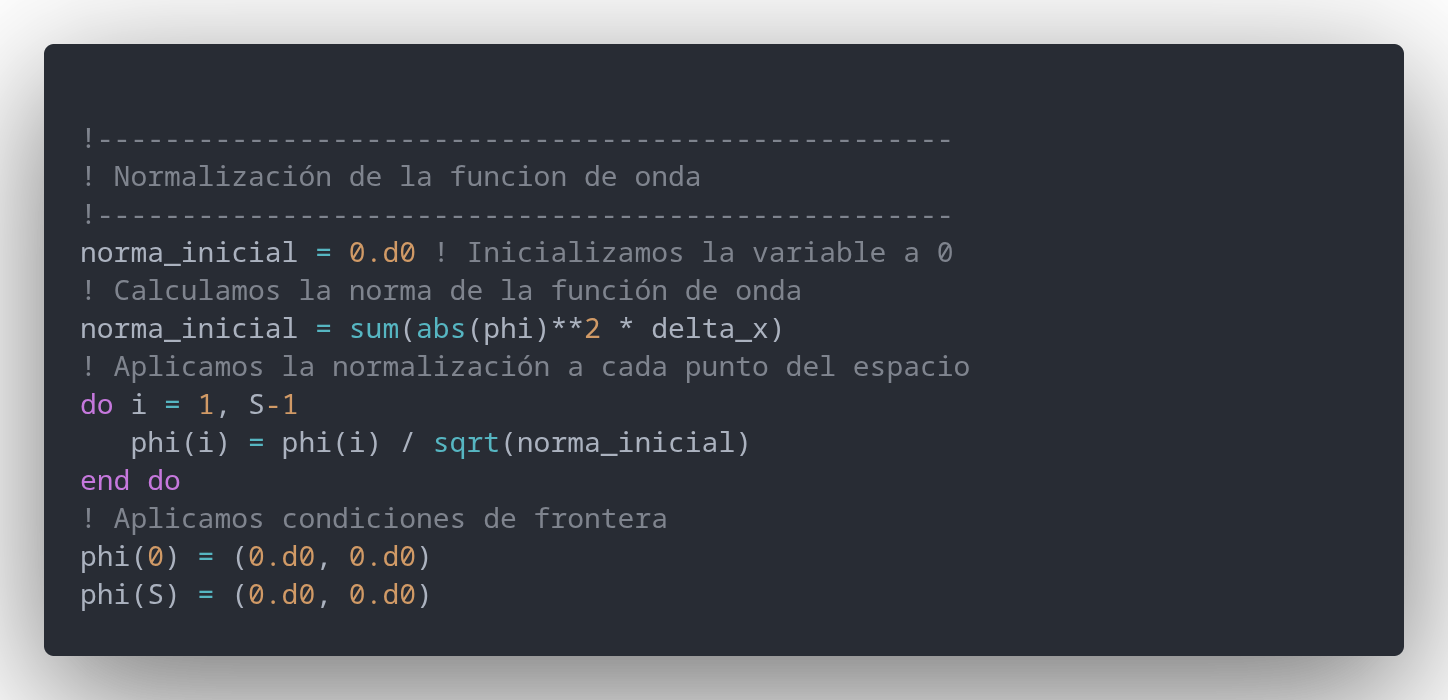
\includegraphics[width=0.8\linewidth]{Image/Code/Norma.png}}
    \caption{Codigo para la normalización de la función de onda en el tiempo inicial.}
    \label{fig:codigo_norma}
\end{figure}

Al obtener la función de onda normalizada en el tiempo inicial, se ha calculado la norma de la función de onda en cada paso de tiempo, obteniendo así la siguiente gráfica:

\begin{figure}[H]
    \centering{
    
\includegraphics[width=0.8\linewidth]{Video/Auto/n_4/simulacion_Norma.png}}
    \caption{Evolución de la norma de la función de onda a lo largo del tiempo.}
    \label{fig:auto_norm}
\end{figure}

Como se puede observar en la gráfica \ref{fig:auto_norm}, la norma de la función de onda se mantiene constante a lo largo del tiempo, lo que confirma que el método de Crank-Nicolson garantiza la conservación de la norma de la función de onda durante la evolución temporal.
\subsubsection{Evolución de la probabilidad}

En esta sección expondremos la evolución de la probabilidad a lo largo del tiempo, para ello se ha calculado la probabilidad de encontrar la partícula en cada punto del espacio en cada paso de tiempo, para ello se ha utilizado la expresión de la probabilidad $P(x,t) = |\psi(x,t)|^2$, obteniendo así la siguiente gráfica:

\begin{figure}[H]
    \centering

    \href{https://wetzap.github.io/Propuestos_Compua/Opcional_Schro/Video/Auto/n_4/simulacion_Phi_Prob.mp4}{
    
\includegraphics[width=0.8\linewidth]{Video/Auto/n_4/simulacion_Phi_Prob_captura.png}
    }
    \caption{Evolución de la probabilidad a lo largo del tiempo.}
    \label{fig:auto_time}
\end{figure}

En la gráfica se expone la evolución tanto clásica como cuántica, la parte clasica la explicaremos en una sección más adelante. En la parte cuántica se puede observar que la probabilidad de encontrar la partícula en cada punto del espacio se mantiene constante a lo largo del tiempo, lo que es consistente con el hecho de que las autofunciones del oscilador armónico cuántico son estados estacionarios, es decir, que no cambian su forma a lo largo del tiempo, aunque si pueden cambiar su fase, que es lo que se observa en la parte real e imaginaria de la función de onda, que se muestra en la siguiente sección, pero, esta variación de la fase no afecta a la probabilidad, ya que esta depende del módulo cuadrado de la función de onda, lo que confirma que las autofunciones del oscilador armónico cuántico son estados estacionarios.




\subsubsection{Parte real e imaginaria de la función de onda}
En esta sección se ha calculado la parte real e imaginaria de la función de onda en cada paso de tiempo, para ello se usarón las funciones de real() y aimag() de Fortran. En la siguiente gráfica se muestra la evolución de la parte real e imaginaria de la función de onda a lo largo del tiempo:


\begin{figure}[H]
    \centering

    \href{https://wetzap.github.io/Propuestos_Compua/Opcional_Schro/Video/Auto/n_4/simulacion_Juntos.mp4}{
    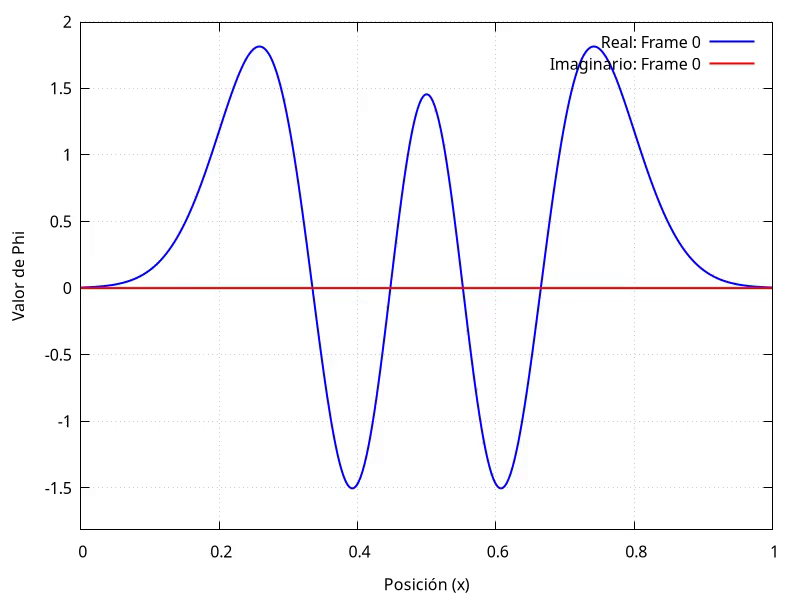
\includegraphics[width=0.8\linewidth]{Video/Auto/n_4/simulacion_Juntos_captura.png}
    }
    \caption{Evolución de la parte real e imaginaria de la función de onda a lo largo del tiempo.}
    \label{fig:auto_re_im}
\end{figure}

Como se observa en la gráfica comenzamos con una parte imaginaria nula y toda la función de onda es real, esto debido a que las autofunciones del sistema son reales. 


\subsubsection{Valor medio de $x$ y $p$}
En esta sección se ha calculado el valor medio de la posición $x$ y el momento $p$ en cada paso de tiempo, además se han comparado con los valores teóricos correspondientes a las autofunciones del oscilador armónico cuántico, para ello se han utilizado las siguientes expresiones teóricas (de nuevos sacadas de \cite{SolucionSchro}) :
\begin{equation}
    \langle x \rangle = \int_{-\infty}^{\infty} x |\psi(x,t)|^2 dx
\end{equation}

\begin{equation}
    \langle p \rangle = -i \int_{-\infty}^{\infty} \psi^*(x,t) \dfrac{\partial}{\partial x} \psi(x,t) dx
\end{equation}

Para el valor medio de $x$ y $p$ en las autofunciones del oscilador armónico cuántico obtendremos los siguientes resultados teóricos:
\begin{equation}
    \langle x \rangle_n =  \langle y \rangle_n + 0.5
\end{equation}
Donde $\langle y \rangle_n$ es el valor medio de $y$ en las autofunciones, el cual, es igual a $0\ \forall n$; por lo que el valor medio de $x$ en las autofunciones del oscilador armónico cuántico es igual a $0.5$ para todas las autofunciones.

\begin{equation}
    \langle p \rangle_n = 0
\end{equation}

Para el calculo numérico del valor medio de $x$ y $p$, se han utilizado los equivalentes discretizados de las expresiones teóricas, a continuación se muestra la aplicación en nuestro programa:

\begin{figure}[H]
    \centering{
    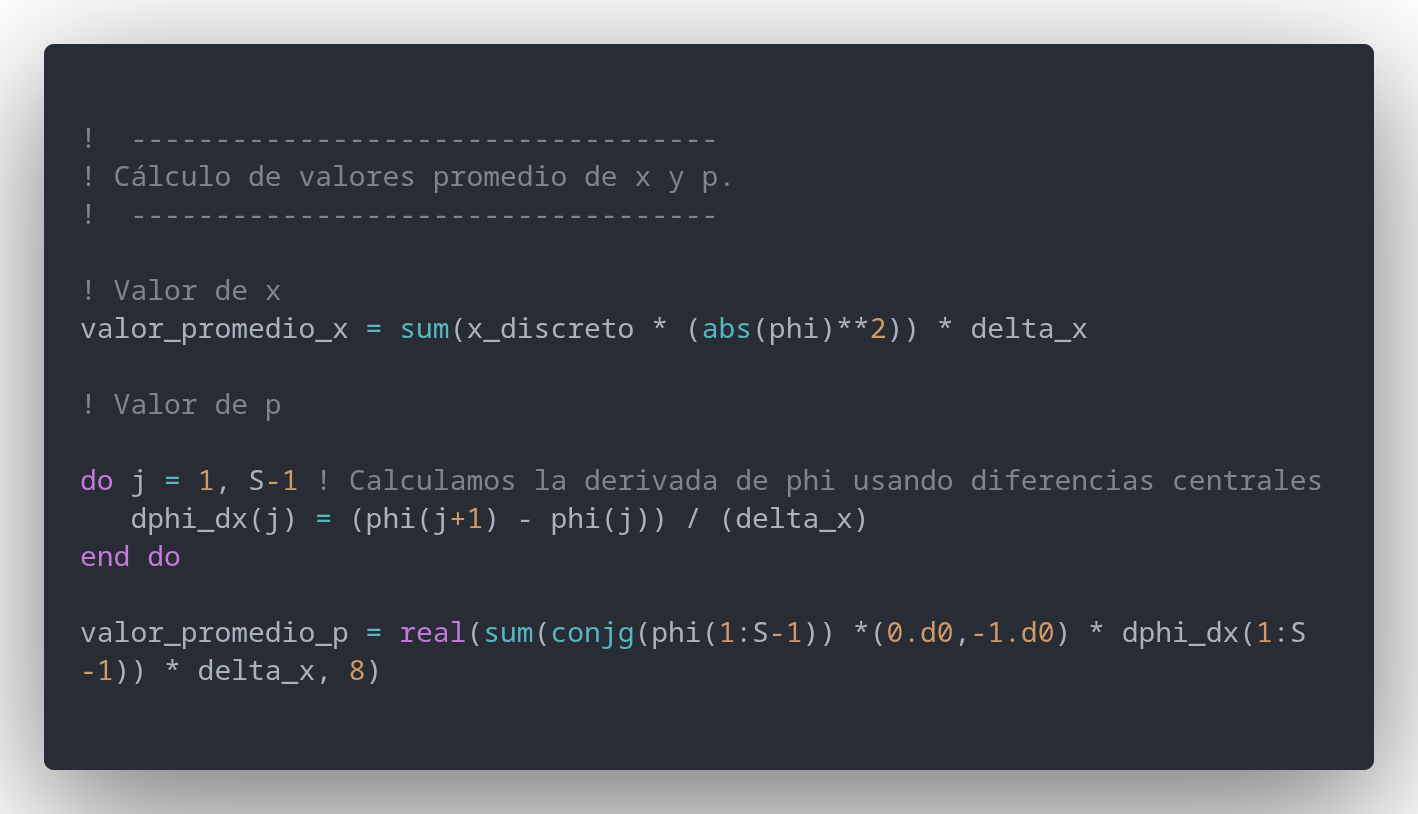
\includegraphics[width=0.8\linewidth]{Image/Code/Valor_Medio.png}}
    \caption{Código para el cálculo del valor medio de $x$ y $p$.}
    \label{fig:codigo_valor_medio}
\end{figure}

Los resultados obtenidos para el valor medio de $x$ y $p$ se muestran en la siguiente gráfica:
\begin{figure}[H]
    \centering{
    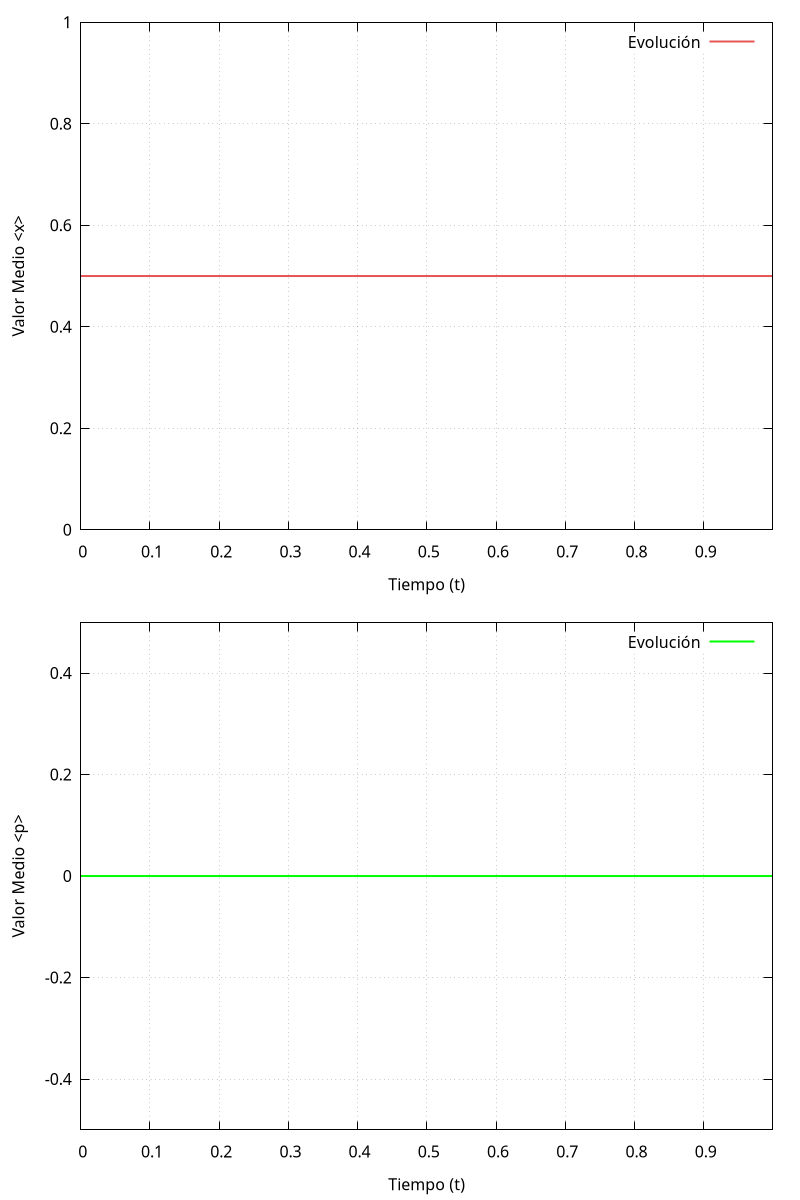
\includegraphics[width=0.8\linewidth]{Video/Auto/n_4/Resumen_Valor_Medio.png}}
    \caption{Evolución del valor medio de $x$ y $p$ a lo largo del tiempo.}
    \label{fig:auto_valor_medio}
\end{figure}

Como se puede observar en la gráfica \ref{fig:auto_valor_medio}, el valor medio de $x$ se mantiene constante en $0.5$ a lo largo del tiempo, mientras que el valor medio de $p$ se mantiene constante en $0$, lo que también es consistente con el hecho de que las autofunciones del oscilador armónico cuántico son estados estacionarios, ya que no hay movimiento neto en el sistema, lo que confirma que las autofunciones del oscilador armónico cuántico son estados estacionarios.

\subsubsection{Principio de incertidumbre y valor medio de $H$}

En esta sección se ha calculado el valor medio de la energía $H$ y el producto de las incertidumbres $\Delta x \Delta p$ en cada paso de tiempo, además se han comparado con los valores teóricos correspondientes a las autofunciones del oscilador armónico cuántico, para ello se han utilizado las siguientes expresiones teóricas (de nuevos sacadas de \cite{SolucionSchro}) :
\begin{equation}
    \langle H \rangle = \int_{-\infty}^{\infty} \psi^*(x,t) \hat{H} \psi(x,t) dx = E_n = \omega (n + \dfrac{1}{2})
\end{equation}

\begin{equation}
    \Delta x \Delta p = \sqrt{\langle x^2 \rangle - \langle x \rangle^2} \sqrt{\langle p^2 \rangle - \langle p \rangle^2} = (n + \dfrac{1}{2})
\end{equation}


Para el calculo numérico del valor medio de $H$ y el producto de las incertidumbres $\Delta x \Delta p$, se han utilizado los equivalentes discretizados de las expresiones teóricas, a continuación se muestra la aplicación en nuestro programa:

\begin{figure}[H]
    \centering{
    
\includegraphics[width=0.8\linewidth]{Image/Code/Valor_MedioH_Incerti.png}}
    \caption{Código para el cálculo del valor medio de $H$ y el producto de las incertidumbres $\Delta x \Delta p$.}
    \label{fig:codigo_valor_medio_H}
\end{figure}

Los resultados obtenidos para el valor medio de $H$ y el producto de las incertidumbres $\Delta x \Delta p$ se muestran en la siguiente gráfica:
\begin{figure}[H]
    \centering{
    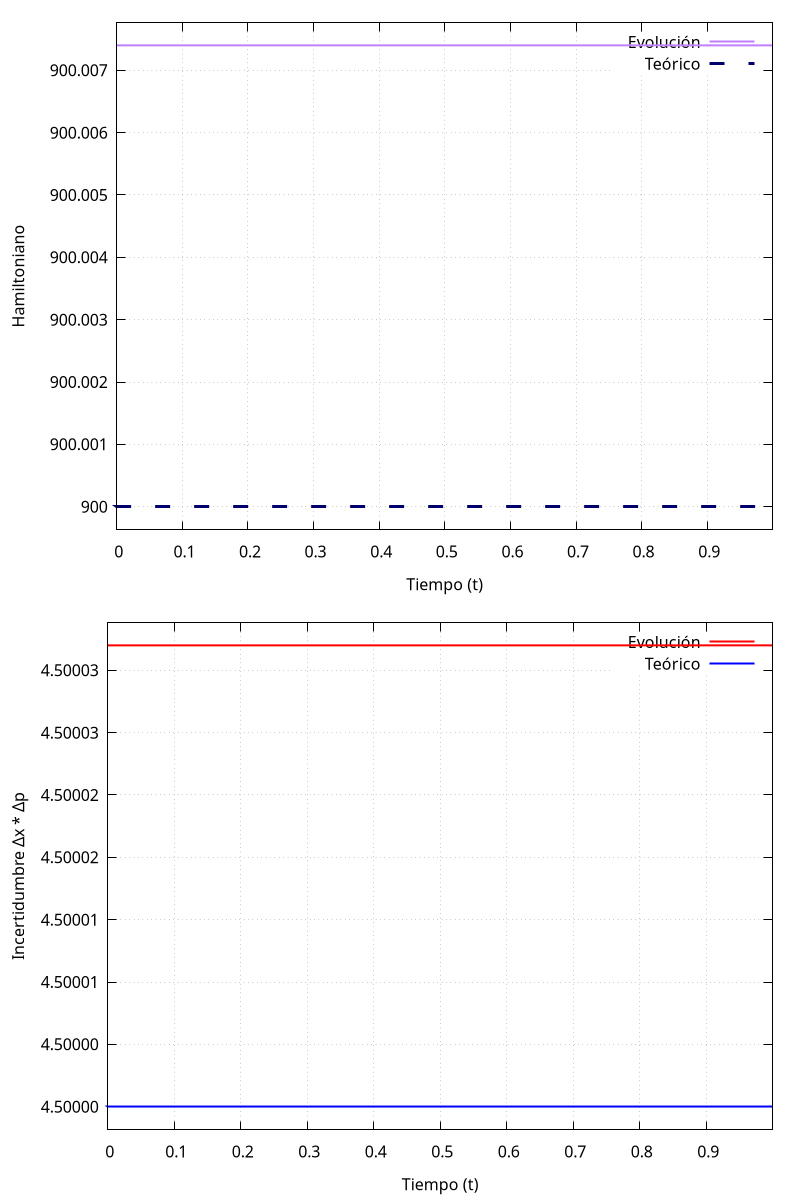
\includegraphics[width=0.8\linewidth]{Video/Auto/n_4/Resumen_Temporal.png}}
    \caption{Evolución del valor medio de $H$ y el producto de las incertidumbres $\Delta x \Delta p$ a lo largo del tiempo.}
    \label{fig:auto_valor_medio_H}
\end{figure}

Como se puede observar en la gráfica \ref{fig:auto_valor_medio_H}, el valor medio de $H$ se mantiene constante en $\omega (n + \dfrac{1}{2})$ a lo largo del tiempo, mientras que el producto de las incertidumbres $\Delta x \Delta p$ se mantiene constante en $(n + \dfrac{1}{2})$. Aunque en el resultado de la incertidumbre se pueda observar que el valor numérico es inferior al valor teórico, esto se debe a que el valor numérico se ha calculado a través de la discretización de las expresiones teóricas, lo que introduce un error numérico en el cálculo, aunque este error es pequeño, es suficiente para que el valor numérico sea inferior al valor teórico.



\subsection{Función Inicial Gaussiana}
En esta sección se ha utilizado una función gaussiana como función de onda inicial, para ello se ha utilizado la siguiente expresión para la función gaussiana:
\begin{equation}
    \psi(x,t_0) = e^{-\dfrac{(x-x_0^{gauss})^2}{2\sigma^2}} \rightarrow \text{discretización} \rightarrow \psi_j^0 = e^{-\dfrac{(j\Delta x-x_0^{gauss})^2}{2\sigma^2}}
\end{equation}

En nuestro caso usaremos el valor de $\sigma = 1.0/16$ y $x_0^{gauss} = 0.3$, manteniendo el resto de parámetros iguales a los utilizados en la sección anterior.
\subsubsection{Conservación de la norma de la función de onda}
Al igual que en la sección de las autofunciones, se ha calculado la norma de la función de onda en cada paso de tiempo para comprobar que se mantiene constante a lo largo del tiempo, obteniendo así la siguiente gráfica:


\begin{figure}[H]
    \centering{
    
\includegraphics[width=0.8\linewidth]{Video/Func/simulacion_Norma.png}
    }
    \caption{Evolución de la norma de la función de onda a lo largo del tiempo.}
    \label{fig:schrodinger_norm}
\end{figure}

Observandose de nuevo que la norma de la función de onda se mantiene constante a lo largo del tiempo, lo que confirma que el método de Crank-Nicolson garantiza la conservación de la norma de la función de onda durante la evolución temporal, incluso para funciones de onda que no son autofunciones del sistema, como es el caso de la función gaussiana utilizada en esta sección.

\subsubsection{Evolución de la probabilidad}

En esta sección se ha calculado la evolución de la probabilidad a lo largo del tiempo para la función gaussiana, obteniendo así la siguiente gráfica:

\begin{figure}[H]
    \centering

    \href{https://wetzap.github.io/Propuestos_Compua/Opcional_Schro/Video/Func/simulacion_Phi_Prob.mp4}{
    
\includegraphics[width=0.8\linewidth]{Video/Func/simulacion_Phi_Prob_captura.png}
    }
    \caption{Evolución de la probabilidad a lo largo del tiempo para la función gaussiana.}
    \label{fig:schrodinger_time}
\end{figure}

La gráfica que muestra la evolución de la probabilidad a lo largo del tiempo para nuestra funcón gaussiana, muestra un comportamiento oscilatorio, comportamiento que no presentaban las autofunciones del oscilador armónico cuántico, esto se debe a que la función gaussiana no es un estado estacionario del sistema, lo que significa que su forma cambia a lo largo del tiempo, lo que se refleja en la evolución de la probabilidad, aunque esta evolución es oscilatoria, la probabilidad de encontrar la partícula en cada punto del espacio se mantiene constante a lo largo del tiempo. 

Además de mostrar la evolución de la probabilidad se ha mostrado la e trayectoria que seguía el maximo de la probabilidad a lo largo del tiempo, mostrando así el comportamiento oscilatorio de la función gaussiana, aunque esta evolución es oscilatoria, la probabilidad de encontrar la partícula en cada punto del espacio se mantiene constante a lo largo del tiempo.


\subsubsection{Parte real e imaginaria de la función de onda}

En esta sección se ha calculado la parte real e imaginaria de la función de onda en cada paso de tiempo para la función gaussiana de igual forma que en la sección anterior, obteniendo así la siguiente gráfica:

\begin{figure}[H]
    \centering
    \href{https://wetzap.github.io/Propuestos_Compua/Opcional_Schro/Video/Func/simulacion_Juntos.mp4}{
    
\includegraphics[width=0.8\linewidth]{Video/Func/simulacion_Juntos_captura.png}
    }
    \caption{Evolución de la parte real e imaginaria de la función de onda a lo largo del tiempo.}
    \label{fig:schrodinger_time}
\end{figure}

Al igual que en la sección de las autofunciones, comenzamos con una parte imaginaria nula y toda la función de onda es real, esto debido a que la función gaussiana utilizada como función de onda inicial es real. A lo largo del tiempo, tanto la parte real como la parte imaginaria de la función de onda evolucionan, mostrando un comportamiento oscilatorio, lo que refleja el hecho de que la función gaussiana no es un estado estacionario del sistema, aunque esta evolución es oscilatoria, la probabilidad de encontrar la partícula en cada punto del espacio se mantiene constante a lo largo del tiempo, lo que confirma que la función gaussiana no es un estado estacionario del sistema.


\subsubsection{Valor medio de $x$ y $p$}

En esta sección se ha calculado el valor medio de la posición $x$ y el momento $p$ en cada paso de tiempo para la función gaussiana, obteniendo así la siguiente gráfica:

\begin{figure}[H]
    \centering
    
\includegraphics[width=0.8\linewidth]{Video/Func/Resumen_Valor_Medio.png}
    \caption{Evolución del valor medio de $x$ y $p$ a lo largo del tiempo.}
    \label{fig:gaus_medio_x_p}
\end{figure}

Como se puede observar en la gráfica \ref{fig:gaus_medio_x_p}, el valor medio de $x$ y $p$ muestran un comportamiento oscilatorio a lo largo del tiempo. Este comportamiento oscilatorio se debe a que la función gaussiana no es un estado estacionario del sistema, lo que significa que su forma cambia a lo largo del tiempo, lo que se refleja en la evolución de los valores medios de $x$ y $p$. Aunque esta evolución es oscilatoria.
\subsubsection{Principio de incertidumbre y valor medio de $H$}

En esta sección se ha calculado el valor medio de la energía $H$ y el producto de las incertidumbres $\Delta x \Delta p$ en cada paso de tiempo para la función gaussiana, obteniendo así la siguiente gráfica:
\begin{figure}[H]
    \centering
    
\includegraphics[width=0.8\linewidth]{Video/Func/Resumen_Temporal.png}
    \caption{Evolución del valor medio de $H$ y el producto de las incertidumbres $\Delta x \Delta p$ a lo largo del tiempo.}
    \label{fig:gaus_energia_incertidumbre}
\end{figure}

Como se puede observar en la gráfica \ref{fig:gaus_energia_incertidumbre}, el valor medio de $H$ muestra una concordancia con el valor teórico de $H$ para la función gaussiana, aunque se puede observar que el valor numérico es ligeramente inferior al valor teórico, esto se debe al error numérico asociado. Además, el producto de las incertidumbres $\Delta x \Delta p$ muestra un comportamiento oscilatorio a lo largo del tiempo, aunque se mantiene por encima del valor teórico de $1/2$, lo que confirma que la función gaussiana cumple con el principio de incertidumbre de Heisenberg.

Puede apreciarse que el principio de incertidumbre oscila a lo largo del tiempo, como si el sistema estuviera respirando, aumentando y disminuyendo  su valor.

\subsection{Comparación con modelo Clásico}

Para las autofunciones del oscilador armónico cuántico, se ha comparado la probabilidad de encontrar la partícula en cada punto del espacio a lo largo del tiempo con el comportamiento clásico del oscilador armónico, para ello se ha utilizado la expresión propuesta en \cite{Bransden2000}, que nos dá la siguiente expresión:

\begin{equation}
    P_c(x) dx = \dfrac{dx}{\pi \sqrt{(x_c^2 - x^2)}}
\end{equation}

Donde $x_c = \sqrt{2E_n/m\omega^2} = \sqrt{4 E_n/\omega^2}$ y $ x= x - x_0$, con $E_n$ el valor de la energía correspondiente a la autofunción utilizada, $m$ la masa de la partícula y $\omega$ la frecuencia del oscilador armónico. Esta expresión nos dá la probabilidad de encontrar la partícula en cada punto del espacio para el modelo clásico del oscilador armónico, esta expresión se ha utilizado para comparar con la evolución de la probabilidad obtenida para las autofunciones del oscilador armónico cuántico, mostrando así las diferencias entre el comportamiento clásico y el comportamiento cuántico del sistema.

Conforme aumentamos el valor de $n$ de las autofunciones, la evolución de la probabilidad obtenida para las autofunciones del oscilador armónico cuántico se acerca cada vez más a la expresión propuesta para el modelo clásico del oscilador armónico, lo que refleja el hecho de que a medida que aumentamos el valor de $n$, las autofunciones del oscilador armónico cuántico se acercan cada vez más a los estados clásicos del sistema, lo que confirma la correspondencia entre el comportamiento clásico y el comportamiento cuántico del sistema, esto se muestra para el valor  de  $n = 20$ en la siguiente gráfica:

\begin{figure}[H]
    \centering

    \href{https://wetzap.github.io/Propuestos_Compua/Opcional_Schro/Video/Auto/n_20/simulacion_Phi_Prob.mp4}{
    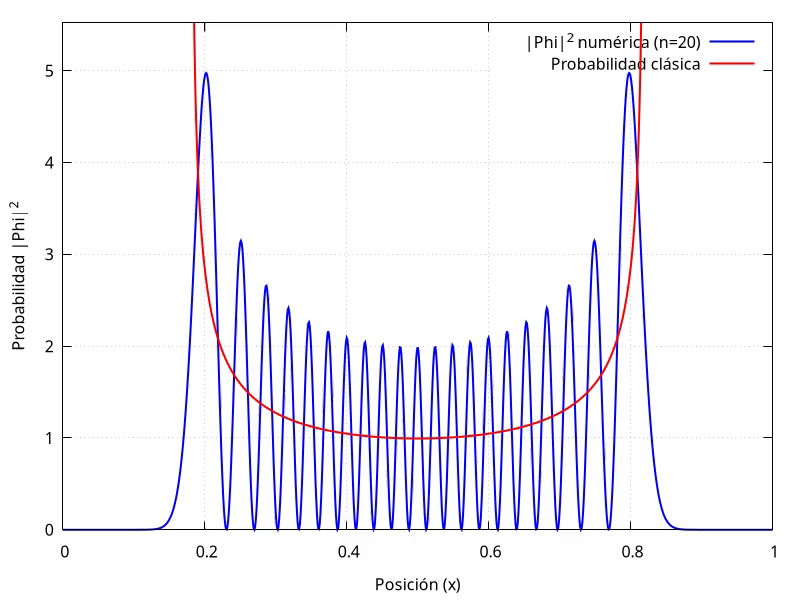
\includegraphics[width=0.8\linewidth]{Video/Auto/n_20/simulacion_Phi_Prob_captura.png}
    }
    \caption{Evolución de la probabilidad a lo largo del tiempo.}
    \label{fig:auto_time_n20}
\end{figure}
En este caso el valor de $\omega$ lo hemos cambiado a $800$ para que se pueda observar mejor la evolución de la probabilidad, ya que, si escogemos un valor de $\omega$ es bajo la evolución de la probabilidad oscila enormenemente.

Si en vez de escoger $n = 20$ escogemos un valor de $n$ más alto, como es el caso de $n = 80$, la evolución de la probabilidad obtenida para las autofunciones del oscilador armónico cuántico se acerca aún más a la expresión propuesta para el modelo clásico del oscilador armónico, lo que refleja el hecho de que a medida que aumentamos el valor de $n$, las autofunciones del oscilador armónico cuántico se acercan cada vez más a los estados clásicos del sistema, la evolución de la probabilidad obtenida se muestra en la siguiente gráfica, en este caso el valor es $\omega=1500$:


\begin{figure}[H]
    \centering
    \href{https://wetzap.github.io/Propuestos_Compua/Opcional_Schro/Video/Auto/n_80/simulacion_Phi_Prob.mp4}{
    
\includegraphics[width=0.8\linewidth]{Video/Auto/n_80/simulacion_Phi_Prob_captura.png}
    }
    \caption{Evolución de la probabilidad a lo largo del tiempo para $n = 80$.}
    \label{fig:auto_time_n80}
\end{figure}

\subsubsection{Explicación del comportamiento del valor de $\omega$}

El comportamiento oscilante que se osbserva en \ref{fig:auto_time_n20} se puede eliminar si escogemos un valor de $\Delta t$ suficientemente pequeño. Además, el valor de $\omega$ afecta directamente a los resultados de $H_n(\alpha y)$, se comprobó que para valores de $\omega$ bajos, como es el caso de $\omega = 200$, el valor de $H_n(\alpha y)$ multiplicado por el valor de la exponencial que acompaña los polinomios de Hermite sea mucho mayor que si escogemos un valor de $\omega$ alto, como es el caso de $\omega = 800$. 


\Large Modelo Clásico \normalsize\\\\
A continuación se explica el comportamiento clásico del oscilador armónico, para ello se ha utilizado la siguiente expresión para la posición $x(t)$ del oscilador armónico clásico:
\begin{equation}
    x(t) = A \cos(\omega t + \phi) + x_0
\end{equation}

Donde $A$ es la amplitud de la oscilación, $\omega$ es la frecuencia del oscilador armónico, $\phi$ es la fase inicial y $x_0$ es la posición de equilibrio del oscilador armónico. El valor de la amplitud $A$ se ha calculado a partir de la energía correspondiente a la función gaussiana utilizada como función de onda inicial, utilizando la siguiente expresión para la energía del oscilador armónico clásico:
\begin{equation}
    E = \dfrac{1}{2} m \omega^2 A^2 \rightarrow A = \sqrt{\dfrac{2E}{m \omega^2}} = \sqrt{\dfrac{4E}{\omega^2}}
\end{equation}


Si combinamos en una misma gráfica el valor medio de $x$ obtenido para la función gaussiana (con un $x_0 = 0.3$) con la expresión de la posición $x(t)$ del oscilador armónico clásico, obtenemos la siguiente gráfica:

\begin{figure}[H]
    \centering
    {
    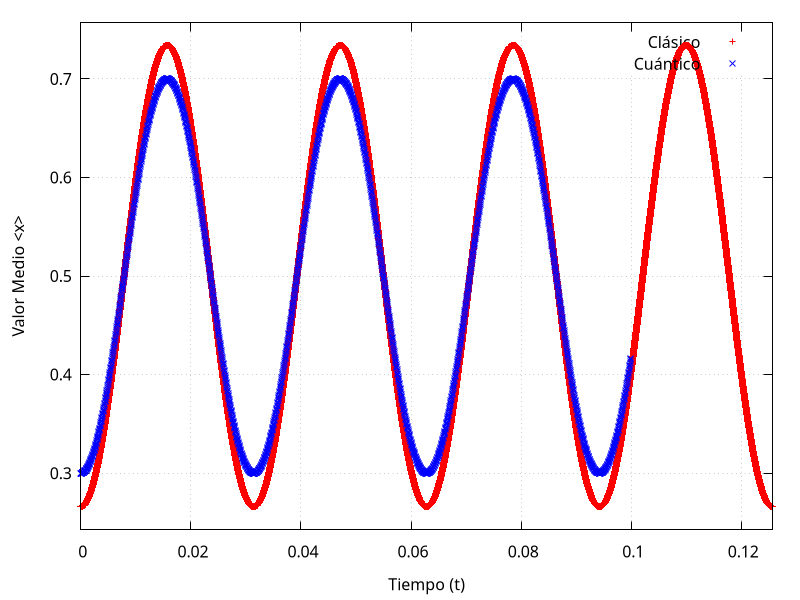
\includegraphics[width=0.8\linewidth]{Video/Clasico/simulacion_clsvscuaPosicion.png}
    }
    \caption{Comparación entre el valor medio de $x$ obtenido para la función gaussiana y la posición $x(t)$ del oscilador armónico clásico.}
    \label{fig:comparacion_clasico_cuantico}
\end{figure}


Y para el momento $p$ obtenemos la siguiente gráfica:

\begin{figure}[H]
    \centering
    {
    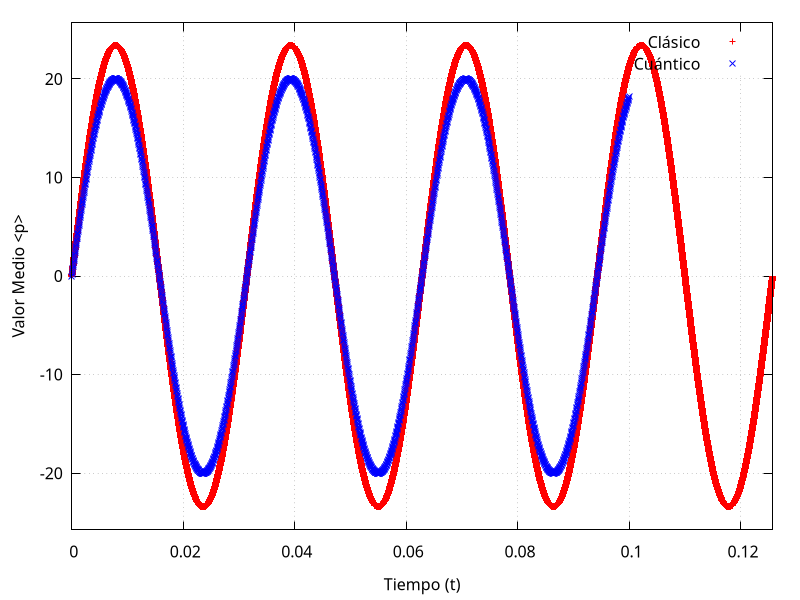
\includegraphics[width=0.8\linewidth]{Video/Clasico/simulacion_clsvscuaMomento.png}
    }
    \caption{Comparación entre el valor medio de $p$ obtenido para la función gaussiana y el momento $p(t)$ del oscilador armónico clásico.}
    \label{fig:comparacion_clasico_cuantico_momento}
\end{figure}


Sin embargo, si cambiamos el valor de $x_0$ de la función gaussiana a $x_0 = 0.5$ y el valor de $\sigma$ a $\sigma = 1/10$,estos cambios hacen que el valor medio de $x$ se desplace y al cambiar el valor de $\sigma$ hacemos que la onda inicial sea más estrecha consiguiendo que la incertidumbre en $p$ sea mayor.Representando el valor medio de $x$ y $p$ para esta nueva función gaussiana, obtenemos la siguiente gráfica:



\begin{figure}[H]
    \centering
    {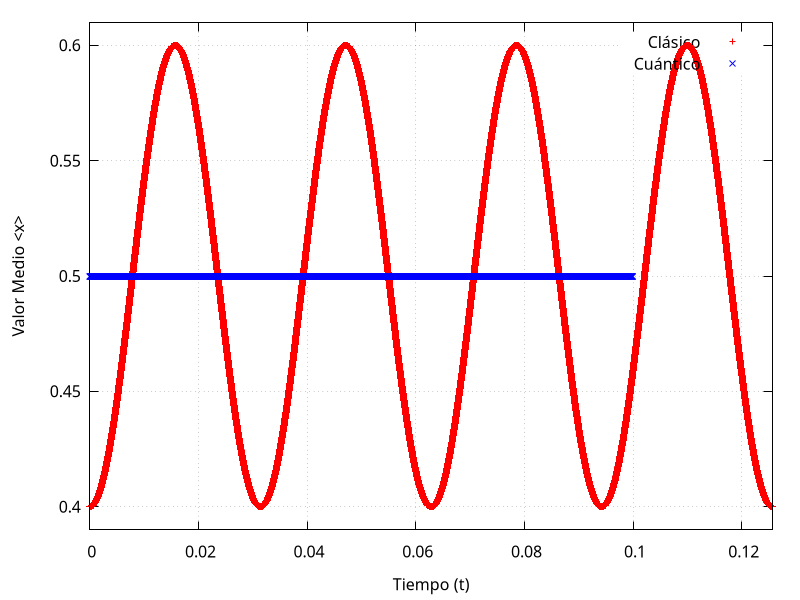
\includegraphics[width=0.8\linewidth]{Video/Clasico/simulacion_clsvscuaPosicion_05.png}}
    \caption{Comparación entre el valor medio de $x$ obtenido para la función gaussiana con $x_0 = 0.5$ y la posición $x(t)$ del oscilador armónico clásico.}
    \label{fig:comparacion_clasico_cuantico_05}
\end{figure}

Y para el momento $p$ obtenemos la siguiente gráfica:

\begin{figure}[H]
    \centering
    {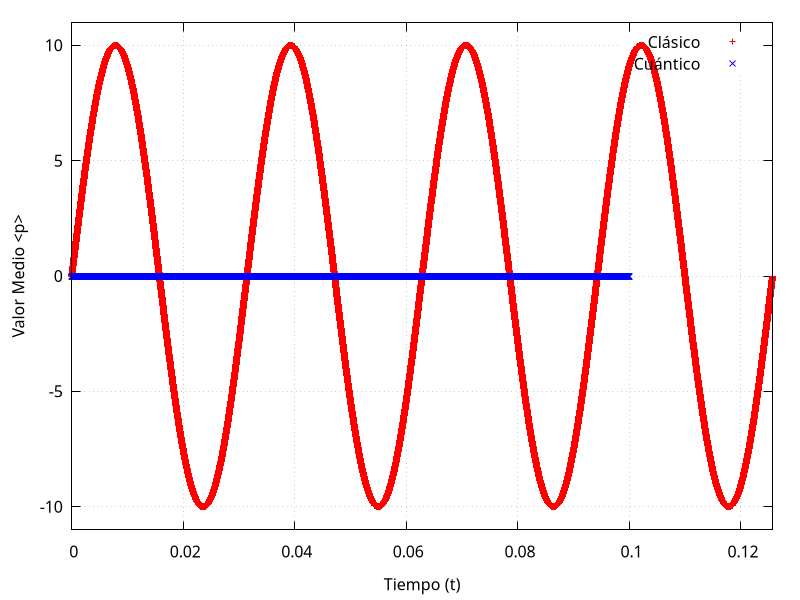
\includegraphics[width=0.8\linewidth]{Video/Clasico/simulacion_clsvscuaMomento_05.png}}
    \caption{Comparación entre el valor medio de $p$ obtenido para la función gaussiana con $x_0 = 0.5$ y el momento $p(t)$ del oscilador armónico clásico.}
    \label{fig:comparacion_clasico_cuantico_momento_05}
\end{figure}


Expliquemos este comportamiento, para ello debemos tener en cuenta que el valor de $x_0$ de la función gaussiana representa la posición de equilibrio del oscilador armónico, por lo que si escogemos un valor de $x_0$ diferente a la posición de equilibrio, como es el caso de $x_0 = 0.3$, la función gaussiana no estará centrada en la posición de equilibrio del oscilador armónico, lo que hará que el valor medio de $x$ muestre un comportamiento oscilatorio a lo largo del tiempo, reflejando el hecho de que la función gaussiana no es un estado estacionario del sistema. 

Sin embargo, si escogemos un valor de $x_0$ igual a la posición de equilibrio, como es el caso de $x_0 = 0.5$, la función gaussiana estará centrada en la posición de equilibrio del oscilador armónico, esto clasicamente hace que su energía sea nula, pero en el caso cuántico, debido al principio de incertidumbre, la función tiene una energía diferente a cero, esto al introducirlo en el caso clásico se refleja en el hecho de que oscile.

Si ahora comparamos los valores del Energía inicial frente a la energía del oscilador, mediante el uso del error relativo obtenemos la siguiente gráfica:

\begin{figure}[H]
    \centering
    {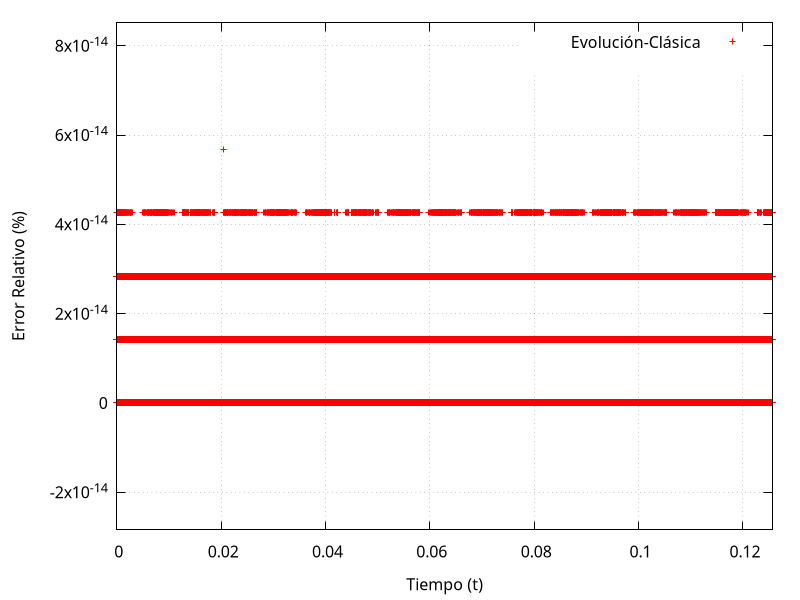
\includegraphics[width=0.8\linewidth]{Video/Clasico/simulacion_cla_Error.png}}
    \caption{Error relativo entre la energía inicial y la energía del oscilador.}
    \label{fig:Energia_relativa}
\end{figure}

Donde se observa un error relativo del orden de $10^{-14}$ lo que confirma que la energía del oscilador armónico clásico es igual a la energía de la función gaussiana, lo que refleja el hecho de que hemos forzado que la energía del oscilador armónico clásico sea igual a la energía de la función gaussiana, lo que hace que el comportamiento del oscilador armónico clásico sea diferente al comportamiento cuántico del sistema, mostrando así las diferencias entre ambos comportamientos.



\section{Conclusiones}

En este trabajo se ha estudiado la evolución temporal de la función de onda para el oscilador armónico cuántico utilizando el método de Crank-Nicolson, se han comparado los resultados obtenidos para las autofunciones del sistema con los resultados obtenidos para una función gaussiana, mostrando así las diferencias entre los estados estacionarios y los estados no estacionarios del sistema. Además, se ha comparado el comportamiento cuántico del sistema con el comportamiento clásico del oscilador armónico, mostrando así la correspondencia entre ambos comportamientos a medida que aumentamos el valor de $n$ de las autofunciones. Finalmente, se ha explicado el comportamiento del valor medio de $x$ y $p$ para la función gaussiana en comparación con el comportamiento clásico del oscilador armónico, mostrando así las diferencias entre ambos comportamientos debido a la naturaleza probabilística del sistema cuántico.


Se han obtenido resultados consistentes con la teoría cuántica, como la conservación de la norma de la función de onda, el comportamiento estacionario de las autofunciones del sistema, y la correspondencia entre el comportamiento clásico y el comportamiento cuántico del sistema a medida que aumentamos el valor de $n$ de las autofunciones. Además, se ha mostrado que el método de Crank-Nicolson es una herramienta útil para estudiar la evolución temporal de la función de onda en sistemas cuánticos, ya que garantiza la conservación de la norma de la función de onda durante la evolución temporal.

\section{Apéndice}
\subsection{Resolución ec. de Schrödinger mediante separación de variables.}
Sea la ecuación de Schrödinger dependiente del tiempo para el oscilador armónico cuántico, la cual se expresa de la siguiente manera:
\begin{equation}
    i\ \dfrac{\partial \Psi(x,t)}{\partial t} = [-\dfrac{\partial^2}{\partial x ^2} + \dfrac{\omega^2}{4}\ (x-0.5)^2]\Psi(x,t) = \hat{H} \Psi(x,t)
\end{equation}

Lo primero que hacemos es suponer que la función de onda $\Psi(x,t)$ se puede escribir como el producto de una función de $x$ y una función de $t$, es decir, $\Psi(x,t) = \psi(x) T(t)$, sustituyendo esta expresión en la ecuación de Schrödinger obtenemos la siguiente expresión:
\begin{equation}
    i\ \psi(x) \dfrac{d T(t)}{dt} = [-\dfrac{d^2}{dx ^2} + \dfrac{\omega^2}{4}\ (x-0.5)^2]\psi(x) T(t)
\end{equation}

Dividiendo ambos lados de la ecuación por $\psi(x) T(t)$ obtenemos la siguiente expresión:
\begin{equation}
    i\ \dfrac{1}{T(t)} \dfrac{d T(t)}{dt} = \dfrac{1}{\psi(x)} [-\dfrac{d^2}{dx ^2} + \dfrac{\omega^2}{4}\ (x-0.5)^2]\psi(x)
\end{equation}

Como el lado izquierdo de la ecuación depende solo de $t$ y el lado derecho depende solo de $x$, ambos lados deben ser iguales a una constante, que denotaremos como $E$, obteniendo así las siguientes ecuaciones:
\begin{equation}
    i\ \dfrac{1}{T(t)} \dfrac{d T(t)}{dt} = E
\end{equation}
\begin{equation}
    \dfrac{1}{\psi(x)} [-\dfrac{d^2}{dx ^2} + \dfrac{\omega^2}{4}\ (x-0.5)^2]\psi(x) = E
\end{equation}

La primera ecuación se puede resolver fácilmente,suponiendo una exponencial compleja como solución, obteniendo la siguiente expresión para $T(t)$:
\begin{equation}
    T(t) = e^{-i E t}
\end{equation}

Para resolver la segunda ecuación, hacemos el cambio de variable $y = x - 0.5$, obteniendo así la siguiente expresión:
\begin{equation}
    [-\dfrac{d^2}{dy ^2} + \dfrac{\omega^2}{4}\ y^2]\psi(y) = E\psi(y) 
\end{equation}

Esta ecuación se resolverá en la los resultados para el caso de la autofunciones \ref{subsec:Autofunciones}


\subsection{Aplicación del método de C-N para la ecuación de Schrödinger (solo discretización temporal).}

Sea la ecuación de Schr. unidimensional con ($\hbar = 1$ y $m = 0.5$):
\begin{equation}
    i\ \dfrac{\partial \Psi(x,t)}{\partial t} = [-\dfrac{\partial^2}{\partial x ^2} + V(x)]\Psi(x,t) = \hat{H} \Psi(x,t)
\end{equation}

La solución formal de esta ecuación incluye el operador de evolución temporal $e^{-i\ (t-t_0)\  H}$, el cual consume una gran cantidad de recursos computacionales, por ello empleamos el método de Crank-Nicholson en una ecución del tipo $\partial_t = -i \hat{H}$. Discretizando el tiempo, obtenemos las siguientes expresiones, dependiendo de si el método es explícito o implícito:

Euler Explícito:
\begin{equation}
    \dfrac{\Psi_{n+1}(x) - \Psi_n(x)}{\Delta t} = -i \hat{H} \Psi^n(x) \Rightarrow \Psi_{n+1}(x) = \Psi_n(x) - i\ \Delta t\ \hat{H} \Psi_n(x)
\end{equation}

Euler Implícito:
\begin{equation}
    \dfrac{\Psi_{n+1}(x) - \Psi_n(x)}{\Delta t} = -i \hat{H} \Psi_{n+1}(x) \Rightarrow \Psi_{n+1}(x) = \Psi_n(x) - i\ \Delta t\ \hat{H} \Psi_{n+1}(x)
\end{equation}

El método de Crank-Nicholson se basa en la media entre ambos métodos, obteniendo así la siguiente expresión:
\begin{equation}
    \dfrac{\Psi_{n+1}(x) - \Psi_n(x)}{\Delta t} = -i \hat{H} \dfrac{\Psi_{n+1}(x) + \Psi_n(x)}{2} \Rightarrow \Psi_{n+1}(x) = \Psi_n(x) - i\ \dfrac{\Delta t}{2}\ \hat{H} [\Psi_{n+1}(x) + \Psi_n(x)]
\end{equation}

Operando sobre la expresion anterior, obtenemos la siguiente ecuación:
\begin{equation}
    (1 + i\ \dfrac{\Delta t}{2}\ \hat{H})\Psi_{n+1}(x) = (1 - i\ \dfrac{\Delta t}{2}\ \hat{H})\Psi_n(x)
\end{equation}

Esta metódo es un método de orden 2, lo que significa que el error de truncamiento es proporcional a $(\Delta t)^2$. Además, es un método incondicionalmente estable, lo que significa que no hay restricciones en el tamaño del paso de tiempo $\Delta t$  garantizando así la estabilidad numérica.

\subsection{Algoritmo de Thomas}

El algoritmo de Thomas es un método eficiente para resolver sistemas de ecuaciones lineales tridiagonales, como el que tenemos en este caso. El algoritmo se basa en la eliminación gaussiana, pero optimizada para aprovechar la estructura tridiagonal del sistema, la expresión general de un sistema de ecuaciones lineales tridiagonal es la siguiente:
\begin{equation}
    a_j x_{j-1} + b_j x_j + c_j x_{j+1} = d_j
\end{equation}

Donde $a_j$, $b_j$ y $c_j$ son los coeficientes de la matriz tridiagonal, $x_j$ son las incógnitas a resolver y $d_j$ son los términos independientes. El algoritmo de Thomas se divide en dos fases: la fase de eliminación hacia adelante y la fase de sustitución hacia atrás.

El sistema de ecuaciones lineales tridiagonal (visto en forma de matriz) que tenemos en este caso es el siguiente:

\begin{equation}
    \begin{bmatrix}
    b_1 & c_1 & 0 & \ldots & 0 \\
    a_2 & b_2 & c_2 & \ldots & 0 \\
    0 & a_3 & b_3 & \ldots & 0 \\
    \vdots & \vdots & \vdots & \ddots & c_{S-1} \\
    0 & 0 & 0 & a_S & b_S
    \end{bmatrix}
    \begin{bmatrix}
    x_1 \\
    x_2 \\
    x_3 \\
    \vdots \\
    x_S
    \end{bmatrix}
    =
    \begin{bmatrix}
    d_1 \\
    d_2 \\
    d_3 \\
    \vdots \\
    d_S
    \end{bmatrix}
\end{equation}


Debido a que solo hay tres diagonales no nulas, el algoritmo hace una pasada hacia adelante para eliminar los términos $a_j$ y luego una pasada hacia atrás para resolver las incógnitas $x_j$. La complejidad computacional del algoritmo de Thomas es $O(n)$, lo que lo hace muy eficiente para resolver sistemas de ecuaciones lineales tridiagonales. Para implementar el algoritmo de Thomas, se siguen los siguientes pasos (estandar):
\begin{enumerate}
    \item Inicialización: Se definen los coeficientes $a_j$, $b_j$, $c_j$ y $d_j$ a partir del sistema de ecuaciones lineales tridiagonal que se desea resolver.
    \item Eliminación hacia adelante: Se realiza una pasada hacia adelante para eliminar los términos $a_j$. Para ello inicialmente se define $c'_1 = c_1 / b_1$ y $d'_1 = d_1 / b_1$. Luego, para cada $j$ desde 2 hasta $S$, se calculan los nuevos coeficientes $c'_j$ y $d'_j$ utilizando las siguientes fórmulas:
    \begin{equation}
        c'_j = \dfrac{c_j}{b_j - a_j c'_{j-1}}
    \end{equation}
    \begin{equation}        d'_j = \dfrac{d_j - a_j d'_{j-1}}{b_j - a_j c'_{j-1}}
    \end{equation}
    \item Sustitución hacia atrás: Se realiza una pasada hacia atrás para resolver las incógnitas $x_j$. Para ello, se define $x_S = d'_S$ y luego, para cada $j$ desde $S-1$ hasta 1, se calcula $x_j$ utilizando la siguiente fórmula:
    \begin{equation}        x_j = d'_j - c'_j x_{j+1}
    \end{equation}
\end{enumerate}



A continuación se muestra el procedimiento que emplearemos nosotros:

\begin{enumerate}
    \item Inicialización: Se definen los coeficientes $a_j$, $b_j$, $c_j$ y $d_j$ a partir del sistema de ecuaciones lineales tridiagonal que se desea resolver.
    \item Linealidad: Usamos un ansatz del tipo $q_{j+1} = \alpha_j q_j + \beta_j$ para eliminar el término, lo introducimos en la ecuación y buscamos la linealidad entre $q_j$ y $q_{j-1}$, obteniendo así las siguientes fórmulas de recurrencia para $\alpha_j$ y $\beta_j$:
    \begin{equation}
        \alpha_{j-1} = -\dfrac{a_j}{b_j + c_j \alpha_j}
    \end{equation}
    \begin{equation}        
        \beta_{j-1} = \dfrac{d_j - a_j \beta_{j}}{b_j + c_j \alpha_j}
    \end{equation}
    \item Sustitución hacia atrás: Se realiza una pasada hacia atrás teniendo en cuenta las condiciones de contorno para los valores iniciales.
\end{enumerate}

\subsection{Aproximación por el método de diferencias centrales.}

Para aproximar la derivada segunda en la ecuación de Schrödinger, se ha utilizado el método de diferencias centrales, la demostración de esta aproximación se puede encontrar en cualquier libro de cálculo numérico, pero a continuación se muestra una breve demostración:

Calculamos la expansion de Taylor de la función $f(x)$ hacia delante y hacia atrás, obteniendo así las siguientes expresiones:
\begin{equation}
    f(x + \Delta x) = f(x) + \Delta x f'(x) + \dfrac{(\Delta x)^2}{2} f''(x) + \dfrac{(\Delta x)^3}{6} f'''(x) + \ldots
\end{equation}
\begin{equation}
    f(x - \Delta x) = f(x) - \Delta x f'(x) + \dfrac{(\Delta x)^2}{2} f''(x) - \dfrac{(\Delta x)^3}{6} f'''(x) + \ldots
\end{equation}

Ahora, sumando ambas expresiones, obtenemos la siguiente expresión:
\begin{equation}
    f(x + \Delta x) + f(x - \Delta x) = 2 f(x) + (\Delta x)^2 f''(x) + 2\dfrac{(\Delta x)^4}{24} f''''(x) + \ldots
\end{equation}

Donde si despejamos $f''(x)$, obtenemos la siguiente expresión:
\begin{equation}
    f''(x) = \dfrac{f(x + \Delta x) - 2 f(x) + f(x - \Delta x)}{(\Delta x)^2} + O((\Delta x)^2)
\end{equation}

Llegando así a la aproximación por el método de diferencias centrales para la derivada segunda, la cual es de orden 2, lo que significa que el error de truncamiento es proporcional a $(\Delta x)^2$.



\subsection{Polinomios de Hermite.}

En esta sección haremos una breve introducción a los polinomios de Hermite, estos polinomios son una familia de polinomios ortogonales, la definición de los polinomios de Hermite es la siguiente:
\begin{equation}
    H_n(x) = (-1)^n e^{x^2} \dfrac{d^n}{dx^n} e^{-x^2}
\end{equation}

Donde $n$ es un número entero no negativo, los polinomios son pares si el valor de $n$ es par y son impares si el valor de $n$ es impar.

Algunos de los primeros polinomios de Hermite son los siguientes:
    \begin{itemize}
        \item $H_0(x) = 1$
        \item $H_1(x) = 2x$
        \item $H_2(x) = 4x^2 - 2$
        \item $H_3(x) = 8x^3 - 12x$
        \item $H_4(x) = 16x^4 - 48x^2 + 12$
        \item $H_5(x) = 32x^5 - 320x^3 + 120x$  
    \end{itemize}

Son polinomios ortogonales con respecto a la función de peso $e^{-x^2}$, lo que significa que cumplen la siguiente relación de ortogonalidad:
\begin{equation}
    \int_{-\infty}^{\infty} e^{-x^2} H_n(x) H_m(x) dx = 0 \quad \text{para} \quad n \neq m
\end{equation}

O si usamos una delta de kronecker:
\begin{equation}
    \int_{-\infty}^{\infty} e^{-x^2} H_n(x) H_m(x) dx = 2^n n! \sqrt{\pi} \delta_{nm}
\end{equation}

Para ampliar la información sobre los polinomios de Hermite, se puede consultar la siguiente referencia \cite{PolinomiosHermite}.



\bibliographystyle{apsrev}
\bibliography{biblio,references}




\end{document}
